%% talk4.tex
%% Copyright 2022 Tom M. Ragonneau
%
% This work may be distributed and/or modified under the
% conditions of the LaTeX Project Public License, either version 1.3
% of this license or (at your option) any later version.
% The latest version of this license is in
%   http://www.latex-project.org/lppl.txt
% and version 1.3 or later is part of all distributions of LaTeX
% version 2005/12/01 or later.
%
% This work has the LPPL maintenance status `maintained'.
%
% The Current Maintainer of this work is Tom M. Ragonneau.
\documentclass{polyu-presentation}
\usepackage{microtype}
\usepackage{booktabs}

% List of hyphenation exceptions for US English
% Source: https://ctan.org/tex-archive/info/digests/tugboat/hyphenex
\input{ushyphex}

% Bibliographical resources
\addbibresource{ragonneau-bib/strings.bib}
\addbibresource{ragonneau-bib/optim.bib}

% Dedicated mathematical macros
\newcommand{\con}[1]{c_{#1}}
\newcommand{\ieq}{\mathcal{E}}
\newcommand{\iub}{\mathcal{I}}
\newcommand{\lag}{\mathcal{L}}
\newcommand{\obj}{f}

\title{Model-Based DFO Methods and Software}
\subtitle[The SQP Method]{Talk no.\ 4 \textemdash\ The SQP Method}
\author[Tom M. Ragonneau]{\texorpdfstring{
    Tom M. Ragonneau\\ 
    \footnotesize Co-supervised by Dr.\ Zaikun Zhang and by Prof.\ Xiaojun Chen
}{Tom M. Ragonneau}}
\institute[PolyU AMA]{
    Department of Applied Mathematics\\
    The Hong Kong Polytechnic University
}
\date{November 21, 2022}
\titlegraphic{}

\begin{document}

\begin{frame}
	\titlepage
\end{frame}

\begin{frame}
    \frametitle{Table of contents}

	\tableofcontents[hideallsubsections]
\end{frame}

\section{Introduction}

\begin{frame}
    \frametitle{The problem}

	We consider
    \begin{align*}
        \min_{x \in \R^n}   & \quad \obj(x)\\
        \text{s.t.}         & \quad \con{i}(x) \le 0, ~ i \in \iub,\\
                            & \quad \con{i}(x) = 0, ~ i \in \ieq,
    \end{align*}
    where derivatives of~$\obj$ and~$\con{i}$ are \alert{known}.
    Recall that its \alert{Lagrangian} is
    \begin{equation*}
        \lag(x, \lambda) = \obj(x) + \sum_{\mathclap{i \in \iub \cup \ieq}} \lambda_i \con{i}(x).
    \end{equation*}

    \begin{block}{The purpose of the SQP method}
        How to \alert{practically} and \alert{efficiently} (Q-quadratically) solve this problem?
    \end{block}
\end{frame}

\section{The SQP method}

\begin{frame}
    \frametitle{A naive idea}

    Given an iterate~$x^k \in \R^n$, let~$d^k$ be an approximate solution to
    \begin{align*}
        \min_{d \in \R^n}   & \quad \obj(x^k) + \nabla \obj(x^k)^{\T} d + \frac{1}{2} d^{\T} \nabla^2 \obj(x^k) d\\
        \text{s.t.}         & \quad \con{i}(x^k) + \nabla \con{i}(x^k)^{\T} d \le 0, ~ i \in \iub,\\
                            & \quad \con{i}(x^k) + \nabla \con{i}(x^k)^{\T} d = 0, ~ i \in \ieq,
    \end{align*}
    and set~$x^{k + 1} = x^k + d^k$.
    
    \medskip

    \begin{block}{}
        \begin{enumerate}[<+(1)->]
            \item It is fairly easy to \alert{implement}.
            \item It generalizes the \alert{Sequential Linear Programming} (SLP) method.
            \item It can only have \alert{local convergence} properties.
            \item But it does \alert{NOT} work\dots
        \end{enumerate}
    \end{block}
\end{frame}

\begin{frame}
    \frametitle{A naive idea (cont'd)}

    Consider
    \begin{align*}
        \min_{x \in \R^2}   & \quad -x_1 - \frac{x_2^2}{4}\\
        \text{s.t.}         & \quad \norm{x}^2 - 1 = 0,
    \end{align*}
    whose \alert{solution} is~$x^{\ast} = [1, 0]^{\T}$.
    Given~$x^k = [t, 0]^{\T}$ with~$t \approx 1$, the subproblem is
    \begin{align*}
        \min_{d \in \R^n}   & \quad -d_1 - \frac{d_2^2}{4}\\
        \text{s.t.}         & \quad d_1 = \frac{1 - t^2}{2t}.
    \end{align*}

    \begin{block}{}
        \begin{enumerate}[<+(1)->]
            \item It is \alert{unbounded from below}, regardless the value of~$t$.
            \item The more~$d^k$ \alert{reduces} the objective function, the \alert{larger}~$\norm{x^k + d^k - x^{\ast}}$ is.
            \item If~$t = 1$, then~$x^k = x^{\ast}$ but~$d^k = 0$ is a \alert{global maximizer}.
        \end{enumerate}
    \end{block}
\end{frame}

\begin{frame}
    \frametitle{The smart idea}

    \begin{block}{What is the problem?}
        The \alert{curvature information} of~$\set{\con{i}}_{i \in \iub \cup \ieq}$ is not represented.
    \end{block}

    \medskip

    The \alert{Sequential Quadratic Programming} (SQP) method solves instead
    \begin{align*}
        \min_{d \in \R^n}   & \quad \obj(x^k) + \nabla \obj(x^k)^{\T} d + \frac{1}{2} d^{\T} H^k d\\
        \text{s.t.}         & \quad \con{i}(x^k) + \nabla \con{i}(x^k)^{\T} d \le 0, ~ i \in \iub,\\
                            & \quad \con{i}(x^k) + \nabla \con{i}(x^k)^{\T} d = 0, ~ i \in \ieq,
    \end{align*}
    with~$H^k \approx \nabla_{x, x}^2 \lag(x^k, \lambda^k)$ for some~$\lambda^k$.

    \medskip

    \begin{block}{}
        \begin{enumerate}
            \item It is as easy to \alert{implement} as before.
            \item It is similar to a \alert{Newton-Raphson} step for the \alert{KKT system}.
        \end{enumerate}
    \end{block}
\end{frame}

\begin{frame}
    \frametitle{A new interpretation}

    We consider here
    \begin{equation*}
        \min_{x \in \R^n} \, \set{\obj(x) : h(x) = 0},
    \end{equation*}
    and for some~$\bar{x}$ and~$\bar{\lambda}$, define
    \begin{equation*}
        Q(d) = \obj(\bar{x}) + \nabla \obj(\bar{x})^{\T} d + \frac{1}{2} d^{\T} \nabla_{x, x}^2 \lag(\bar{x}, \bar{\lambda}) d.
    \end{equation*}
    
    \begin{block}{}
        Consider a curve parametrized by~$x : \R \to \R^n$ satisfying
        \begin{equation*}
            h\big(x(t)\big) = h(\bar{x}) \quad \text{for all~$t \in \R$}, \quad \text{and} \quad x(0) = \bar{x}.
        \end{equation*}

        \smallskip

        \begin{center}
            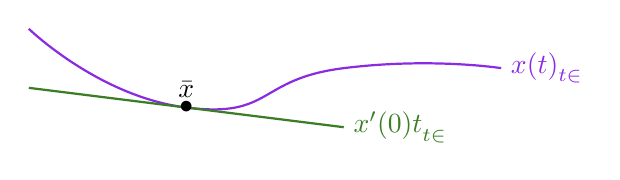
\begin{tikzpicture}
                \draw[thick,BlueViolet] plot[smooth,tension=1] coordinates {(0,0) (2,-1) (4,-0.5) (6,-0.5)};
                \draw[thick,OliveGreen] (0, -0.75) -- (4,-1.25);
                \node at (2,-1) {$\bullet$};
                \node[above] at (2,-1) {$\bar{x}$};
                \node[right,BlueViolet] at (6,-0.5) {$\set{x(t)}_{t \in \R}$};
                \node[right,OliveGreen] at (4,-1.25) {$\set{x'(0)t}_{t \in \R}$};
            \end{tikzpicture}
        \end{center}
    \end{block}
\end{frame}

\begin{frame}
    \frametitle{A new interpretation (cont'd)}

    \begin{block}{}
        Under some \alert{regularity assumptions}, there exist~$\nu \ge 0$ and~$\epsilon > 0$ such that
    \begin{equation*}
        \abs[\big]{f \big( x(t) \big) - Q \big( x'(0) t \big)} \le \bigg( \nu t + \frac{1}{2} \abs[\big]{x''(0)^{\T} \big[ \nabla \obj(\bar{x}) + \nabla h(\bar{x})^{\T} \bar{\lambda} \big]} \bigg) t^2,
    \end{equation*}
    for all~$t \in (-\epsilon, \epsilon)$.
    \end{block}

    \smallskip

    \begin{center}
        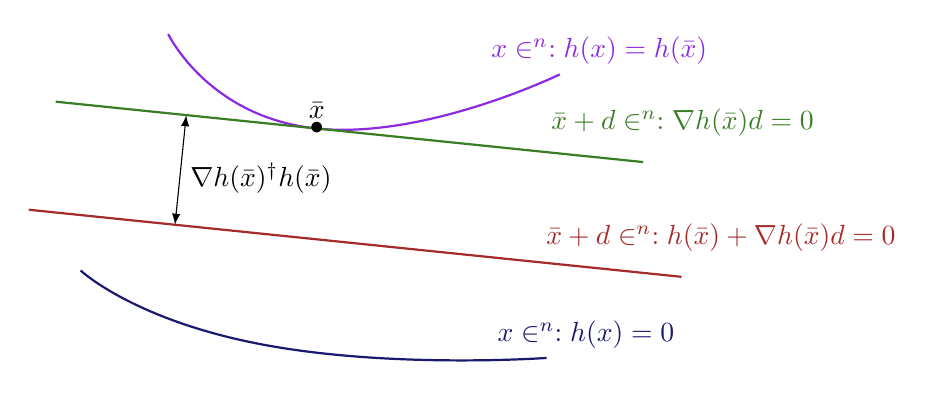
\begin{tikzpicture}[rotate=301]
            \draw[thick,BlueViolet] plot[smooth,tension=1] coordinates {(0,2) (2,3) (3,6)};
            \draw[thick,MidnightBlue] plot[smooth,tension=1] coordinates {(2,-0.5) (4,1) (6,4)};
            \draw[thick,OliveGreen] (0,1/3) -- (4.5,19/3);
            \draw[thick,Brown] (1,-2/3) -- (6,18/3);
            \draw[latex-latex] (1,5/3) -- (53/25,62/75);
    
            \node at (2,3) {$\bullet$};
    
            \node[above] at (2,3) {$\bar{x}$};
            \node[right,yshift=-0.1cm] at (39/25,187/150) {$\norm{\nabla h(\bar{x})^{\dagger} h(\bar{x})}$};
            \node[above,BlueViolet,xshift=0.5cm] at (3,6) {$\set{x \in \R^n : h(x) = h(\bar{x})}$};
            \node[above,OliveGreen,xshift=0.5cm,yshift=0.2cm] at (4.5,19/3) {$\set{\bar{x} + d \in \R^n : \nabla h(\bar{x}) d = 0}$};
            \node[above,Brown,xshift=0.5cm,yshift=0.2cm] at (6,18/3) {$\set{\bar{x} + d \in \R^n : h(\bar{x}) + \nabla h(\bar{x}) d = 0}$};
            \node[above,MidnightBlue,xshift=0.5cm] at (6,4) {$\set{x \in \R^n : h(x) = 0}$};
        \end{tikzpicture}
    \end{center}
\end{frame}

\section{The Maratos effect}

\begin{frame}
    \frametitle{Merit functions}

	\begin{block}{What are merit functions?}
        They measure the \alert{quality} of points by considering both~$\obj$ and~$\set{\con{i}}_{i \in \iub \cup \ieq}$.
    \end{block}

    \medskip

    For example, the~\alert{$\ell_p$-merit functions} are defined for~$x \in \R^n$ by
    \begin{equation*}
        \varphi_{\gamma}(x) = \obj(x) + \gamma \bigg( \sum_{i \in \iub} \posp{\con{i}(x)}^p + \sum_{i \in \ieq} \abs{\con{i}(x)}^p \bigg)^{1/p}, \quad \text{with~$\gamma \ge 0$}.
    \end{equation*}

    \begin{block}{}
        \begin{enumerate}[<+(1)->]
            \item The SQP method must be \alert{globalized} in practice.
            \item This normally requires using \alert{merit functions}.
            \item But this may \alert{jeopardize} fast local convergence\dots
        \end{enumerate}
    \end{block}
\end{frame}

\begin{frame}
    \frametitle{The Maratos effect}

    Consider
    \begin{align*}
        \min_{x \in \R^2}   & \quad 2(\norm{x}^2 - 1) - x_1\\
        \text{s.t.}         & \quad \norm{x}^2 - 1 = 0,
    \end{align*}
    whose \alert{solution} is~$x^{\ast} = [1, 0]^{\T}$.
    Given~$x^k = [\cos t, \sin t]^{\T}$ and~$\lambda^k = 3/2$, we have
    \begin{equation*}
        d^k =
        \begin{bmatrix}
            \sin^2 t\\
            - \cos t \sin t
        \end{bmatrix}
        \quad \text{and} \quad
        \varphi_{\gamma}(x^k + d^k) - \varphi_{\gamma}(x^k) = (1 + \gamma) \sin^2 t \ge 0.
    \end{equation*}

    \begin{block}{}
        \begin{enumerate}[<+(1)->]
            \item The step is \alert{rejected} by any \alert{monotonic} method for any~$\gamma \ge 0$.
            \item It is usually dealt with using \alert{second-order correction} mechanisms.
            \item There exist merit functions that \alert{do not suffer} from the Maratos effect.
        \end{enumerate}
    \end{block}
\end{frame}

\section{Trust-region SQP methods}

\begin{frame}
    \frametitle{Title}

	To do.
\end{frame}

\section{Conclusion}

\begin{frame}
    \frametitle{Title}

	To do.
\end{frame}

\begin{frame}[t,allowframebreaks]
    \frametitle{References}

	\printbibliography
\end{frame}

\end{document}